\documentclass{article}
\usepackage{amsmath}
\usepackage{amssymb}
\usepackage{graphicx}
\usepackage{float}
\usepackage{subcaption}
\usepackage{cleveref}


\newcommand{\showeq}[1]{\text{\eqref{#1}}}
\newcommand{\tr}{\text{tr}}
\begin{document}
	\tableofcontents
	Hello
	\section{Derivation of equations}
	We start with free energy for excluded volume. 
	\begin{equation}\label{free-energy}
		F=\frac{C_{rest}}{C_{\infty}}\left(u\ln\left(\frac{u}{c_{\infty}-u-v}\right)+v\ln\left(\frac{v}{c_{\infty}-u-v}\right)\right)+c_{\infty}\ln\left(1-\frac{u+v}{c_{\infty}}\right)
	\end{equation}
	For the rest of this text I will use $ c $ instead of $ c_{\infty} $. Also I denote
	\begin{equation}
		R = c-u-v, A = \frac{C_{\text{rest}}}{c_\infty}
	\end{equation}
	From free energy we get the chemical potentials
	\begin{align}
		\mu_{u}&=\frac{\partial F}{\partial u}=A\left(\left(\ln\frac{u}{R}\right)+\frac{R+u+v-c_{\infty}}{R}\right)=A\left(\ln\frac{u}{R}\right)= A \ln(u)-A\ln(R) \\
		\mu_{v}&=\frac{\partial F}{\partial v}= = A \ln(v)-A\ln(R)
	\end{align}
	
In the end we want to compute  $\partial_x u \partial_x(\mu_u)$, because the full equation is 
\begin{equation}
\dot{u} = \partial_x u \partial_x(\mu_u) + f_u(u,v).
\end{equation}

 
 
The computations are contained in the next subchapter
	\subsection{Extended calculations}
		We want to compute
	\begin{equation}\label{chemical-potential}
		\mu_{u}=\frac{\partial F}{\partial u},
	\end{equation}
where 
\begin{align}
	F=&u\ln\frac{u}{R}+v\ln\frac{v}{R}+c\ln\left(1-\frac{u+v}{c}\right)\\
	=&u\ln u-u\ln R+v\ln v-v\ln R+c\ln R - c \ln c
\end{align}
We have 
\begin{align*} 
	&\frac{\partial}{\partial u}\left(u \ln u\right) = \ln u + 1, \\ 
	&\frac{\partial}{\partial u}\left(-u \ln R\right) = -\ln R + \frac{u}{R},  \text{ (the mistakes were here)}\\ 
	&\frac{\partial}{\partial u}\left(v \ln v\right) = 0, \\ 
	&\frac{\partial}{\partial u}\left(-v \ln R\right) = \frac{v}{R}, \\ &\frac{\partial}{\partial u}\left(c \ln R\right) = -\frac{c}{R}, \\ &\frac{\partial}{\partial u}\left(-c \ln c\right) = 0. 
\end{align*} 
So in the end we get
\begin{equation}
	\mu_u = \ln u -\ln R = \ln u - \ln (c-u-v),
	\end{equation}	
	using 
	\begin{equation}
	R = c-u-v.
	\end{equation}

Now we compute derivative
We have
\begin{equation}
\partial_{x}\mu_{u}=\frac{u^{\prime}}{u}-\frac{R^{\prime}}{R}=\left(\frac{1}{u}+\frac{1}{R}\right)u^{\prime}+\frac{1}{R}v^{\prime}
\end{equation}
So we would get 
\begin{align}
&D_{uu}=(1+\frac{u}{R})=1+\frac{u}{c-u-v}\\
&D_{uv}=\frac{u}{R}=\frac{u}{c-u-v}
\end{align}

So 
\begin{align}\partial_x( u \partial_x \mu_u) &=u''+ \frac{u'R-R'u}{R^2}(u'+v')+\frac{u}{R}(u''+v'')\\
&=u''+\frac{u'}{R}(u'+v')+\frac{u}{R^2}(u'+v')^2+\frac{u}{R}(u''+v'')\\&=
u''-\frac{u(RR''-(R')^2)+R'u'R}{R^2}\\
&=u'' - \frac{u}{R}R'' + u\frac{(R')^2}{R^2}-\frac{R'u'}{R}
\end{align}
Or finally
\begin{align}
\partial_x( u \partial_x \mu_u)=&u''+\frac{u'}{(c-u-v)}(u'+v')\\&+\frac{u}{(c-u-v)^2}(u'+v')^2+\frac{u}{(c-u-v)}(u''+v'')\label{eq:laplacian}
\end{align}

And from this we get the linearization $u \to u+\delta u$, by also assuming  $u',v',u'',v'' = 0$
and ignoring higher order terms.
$$\delta \dot u = \delta u'' + \frac{u}{c-u-v}(\delta u'' + \delta v'') + \text{ reaction kinetics part}$$
If we introduce the coefficient in free energy we'll get
$$\delta \dot u = D_1\left(\delta u'' + \frac{u}{c-u-v}(\delta u'' + \delta v'')\right) + \text{ reaction kinetics part}$$
Or
$$\delta \dot u = \left(D_{uu}\delta u'' + D_{uv}\delta v'' \right)$$
for $\delta  w=(\delta u, \delta v)$
$$\delta \dot w = \begin{pmatrix} D_1(1+\frac{u}{c-u-v}) & D_1\frac{u}{c-u-v}\\ D_2\frac{v}{c-u-v} & D_2(1+\frac{v}{c-u-v})\end{pmatrix} \delta w'' + \text{ reaction kinetics part}$$
So the end result is the same
		
\subsection{Linearization}
The linearized equation looks like
\begin{equation}
\delta \dot w = \bar{D} \delta w'' + A(w) \delta w,
\end{equation}
where 
\begin{equation}
\bar{D} = \begin{pmatrix} D_1(1+\frac{u}{c-u-v}) & D_1\frac{u}{c-u-v}\\ D_2\frac{v}{c-u-v} & D_2(1+\frac{v}{c-u-v})\end{pmatrix} 
\end{equation}
As usual taking $\delta w = v_q \exp{iqx+\sigma t}$ leads to the eigenvalue problem
\begin{equation}
\sigma v_q = (-q^2 \bar{D}+A)v_q
\end{equation}

\section{Eigenvalue analysis}
We want to find the eigenvalues $\sigma(q)$. Thus we look at the characteristic polynomial
\begin{equation}
\det(A-q^2\bar{D}-\sigma\mathbf{1}) = 0
\end{equation}
We can denote $A_q = A-q^2 \bar{D}$.
Then we get
\begin{equation}
\sigma^2 - \text{tr}A_q \sigma + \det A_q = 0
\end{equation}
with the solutions
\begin{equation}
\sigma=\frac12\left(\text{tr}A_q \pm \sqrt{(\text{tr}A_q)^2-4\det A_q}\right)
\end{equation}
As before the condition for stability is
\[\tr A_q < 0, \det A_q > 0.\]


\subsection{The determinant}
We have the following expresssion for the determinant
\begin{equation}
\det A_q = \det A - q^2(d_{uu}a_{vv}+d_{vv}a_{uu}-d_{uv}a_{vu}-d_{vu}a_{uv})+q^4 \det \bar{D}.
\end{equation}
We'll write this as
\begin{equation}
\det A_q = \det A - Bq^2 + C q^4,
\end{equation}
We can see that
\begin{equation}
C = D_1D_2\frac{c}{c-u-v},
\end{equation}
or
\begin{equation}
\det A_q = \det A - q^2(D_{2}a_{uu}+D_1a_{vv} + B') + q^4 (D_1 D_2 + C'),
\end{equation}
where $B',C'$ are the terms occuring solely due to the interactions.
We find that the minimum occurs at $q_{crit}^2 = \frac {B}{2C}$ and
\begin{equation}
\det A_{q_{crit}} = \det A - \frac{B^2}{4C}
\end{equation}


\subsection{The brusselator}
In the case of Brusselator we have
\begin{align}
A&=\begin{pmatrix}b-1& a^2 \\ -b &-a^2\end{pmatrix}\\
\tr A &= b-1-a^2\\
\det A&= a^2\\
u&=a,v=\frac{b}{a} (\text{fixed point})\\
f_u &= a-(b+1)u+u^2v, f_v = bu-u^2v
\end{align}

\begin{equation}
B=\frac{D_1(2ab-a^2c)+D_2(a-c+bc-2ab)}{R}
\end{equation} or in the case of $D_1 = D_2$
\begin{equation}
B = \frac{a-c+bc-a^2c}{R},
\end{equation}
where $R = c-a-\frac ba$.
Thus
\begin{equation}
\det A_q = a^2 - q^2\frac{D_1(2ab-a^2c)+D_2(a-c+bc-2ab)}{c-a-\frac{b}{a}}+q^4\frac{c}{c-a-\frac{b}{a}}
\end{equation}
The trace is equal to
\begin{equation}
\tr A_q = b-1-a^2 - q^2 (\frac{D_1(c-\frac{b}{a})+D_2(c-a)}{c-a-\frac{b}{a}})
\end{equation}

\subsection{Neutral curves}
To find the neutral curve we set 
$\det A_q = 0$. From this we solve for $b$. 
We get
\begin{equation}
b(q)=\frac{D_1 D_2 c q^4 + D_1 a^2 c q^2 - D_2 a q^2 + D_2 c q^2 - a^3 + a^2 c}{2 D_1 a q^2 - 2 D_2 a q^2 + D_2 c q^2 + a}
\end{equation}
In the case of $D_1=D_2$ it simplifies to
\begin{equation}
b=\frac{D^2 c q^4 +Dq^2(  a^2 c  -  a  +  c ) - a^3 + a^2 c}{D c q^2 + a} 
\end{equation}
It's important to remember that $R>0$ i.e $c-a-\frac{b}{a}>0$, which gives us a bound on $b$.\\
The neutral curve  for trace is more complicated. 
\begin{equation}
0=-b^2 + b \left(a c+D_1 q^2+1\right)+a^4-a^3 c+a^2 \left(D_2 q^2+1\right)-a c D_1 q^2-a c D_2 q^2-a c
\end{equation}

\section{Results}
\subsection{Neutral curve}
Here are some comparisons between neutral curves of det, with and without interactions
\begin{figure}[H]
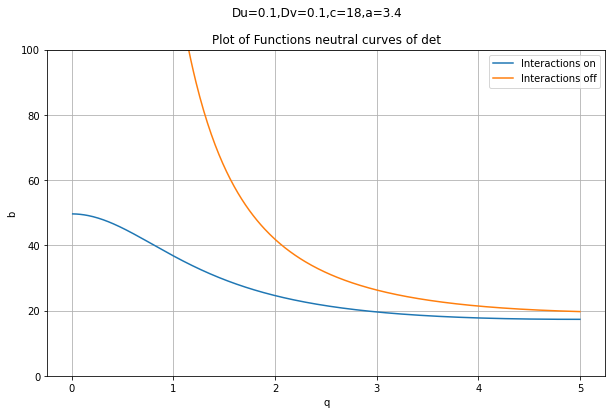
\includegraphics[width=\textwidth]{images/plot_20240719_111506.png} 

\end{figure}
\begin{figure}[H]
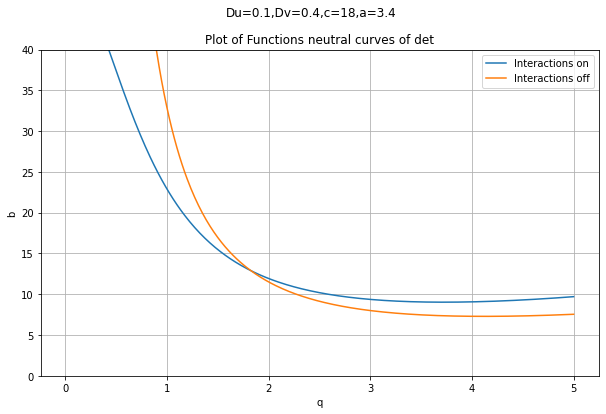
\includegraphics[width=\textwidth]{images/plot_20240719_112606.png} ng

\end{figure}
\section{Collected equations}
\begin{align}
A&=\begin{pmatrix}b-1& a^2 \\ -b &-a^2\end{pmatrix}\\
\tr A &= b-1-a^2\\
\det A&= a^2\\
u&=a,v=\frac{b}{a} (\text{fixed point})\\
f_u &= a-(b+1)u+u^2v, f_v = bu-u^2v
\end{align}

\begin{equation}
\bar{D} = \begin{pmatrix} D_1(1+\frac{u}{c-u-v}) & D_1\frac{u}{c-u-v}\\ D_2\frac{v}{c-u-v} & D_2(1+\frac{v}{c-u-v})\end{pmatrix} 
\end{equation}

	\begin{equation}
	\det A_{q}=\det A-q^2\left(d_{uu}a_{vv}+d_{vv}a_{uu}-a_{vu}d_{uv}-d_{vu}a_{uv}\right)+q^4 \det \bar{D},
	\end{equation}
	
	\begin{equation}
	\tr A_q = \tr A - q^2 (D_1 (1+\frac uR) + D_2 (1+\frac vR)
	\end{equation}
	
	\begin{equation}
	C = D_1D_2 \frac{c}{R}
	\end{equation}
	
\end{document}